\documentclass{beamer}
\usepackage[utf8]{inputenc}

\usetheme{Madrid}
\usecolortheme{default}

%% packages
\usepackage{hyperref}
\newcommand{\email}[1]{\href{mailto:#1}{\nolinkurl{#1}}}
\usepackage{xspace}
\usepackage{xcolor}
\usepackage{graphicx}
\usepackage{amsmath, amssymb, amsthm}
\usepackage{tikz}
\definecolor{dgray}{RGB}{160,160,160}
\definecolor{lgray}{RGB}{235,235,235}
\usetikzlibrary{chains, arrows, positioning}
\usepackage{booktabs}
\newcommand{\ra}[1]{\renewcommand{\arraystretch}{#1}}
\usepackage{array}
\usepackage[edges]{forest}
\usepackage{algorithm}
\usepackage{algorithmic}
\renewcommand{\algorithmicrequire}{\textbf{Input:}}
\usepackage{multirow}
\usepackage{multicol}

\usepackage{makecell}

\newcommand{\bx}{\mathbf{x}}
\newcommand{\vx}{\mathbf{x}}
\newcommand{\bz}{\mathbf{z}}
\newcommand{\vz}{\mathbf{z}}
\newcommand{\bI}{\mathbf{I}}
\newcommand{\beps}{\bm{\epsilon}}
\newcommand{\softmax}{\mathrm{softmax}}
\newcommand{\E}{\mathbb{E}}
\newcommand{\cL}{\mathcal{L}}
\newcommand{\z}[1]{\bz_{t({#1})}}
\newcommand{\zs}[1]{\bz_{s({#1})}}
\newcommand{\kl}{\mathrm{KL}}
\newcommand{\KL}[2]{\mathrm{KL}({#1}\|{#2})}
\newcommand{\snr}{\text{SNR}}
\newcommand{\twonorm}[1]{\|{#1}\|_2}
\newcommand{\diff}{\mathop{}\!\mathrm{d}}

%------------------------------------------------------------
% Title page configuration
%------------------------------------------------------------

\title[Block Diffusion]{Block Diffusion: Interpolating Between Autoregressive and
Diffusion Language Models}

\author[Team 6]{ Ntountounakis Georgios, Markoulidakis Georgios, Vitalis Petros,
Makras Ilias, Kritharidis Konstantinos, Kordas Nikolaos}

\institute[NTUA]
{ Pattern Recognition, ECE\\ National Technical University of Athens }

\date[January 2026]{January 2026}

\AtBeginSection[]{
    \begin{frame}
        \frametitle{Table of Contents}
        \tableofcontents[currentsection]
    \end{frame}
}

\AtBeginSubsection[]{
    \begin{frame}
        \frametitle{Table of Contents}
        \tableofcontents[currentsection,currentsubsection]
    \end{frame}
}

\begin{document}
    \frame{\titlepage}

    \begin{frame}
        \frametitle{Table of Contents}
        \tableofcontents
    \end{frame}

    \section{Paper Overview}
    
    \begin{frame}{Introduction to the Problem-Motivation}
        \textbf{Two main approaches for Language Models:}

        \vspace{0.3cm}
        \begin{columns}
            \column{0.5\textwidth}
            \textbf{Autoregressive (AR):}
            \begin{itemize}
                \item Token-by-token generation %Σειριακή εξάρτηση των δεδομένων%

                \item High quality %Κάπου εδώ να αναφερθεί τι είναι το perplexity%

                \item KV caching %Αποφυγή επανυπολογισμού των key και value vectos στο attention, πρέπει να το αναφέρουμε σίγουρα προφορικά ίσως και γραπτά%

                \item Variable length
            \end{itemize}

            \column{0.5\textwidth}
            \textbf{Diffusion:}
            \begin{itemize}
                \item Parallel generation % Η πιθανότητα κάθε θέσης ανεξάρτητη από τις άλλες - σε αντίθεση με τη σειριακή εξάρτηση πριν - ταυτόχρονο generation

                \item Better controllability

                \item \textcolor{red}{Fixed length (limitation)}

                \item \textcolor{red}{Lower quality (Perplexity Gap)}
                % Γιατί τα παραπάνω 3?
            \end{itemize}
        \end{columns}

        \vspace{0.5cm}
        {
        \begin{alertblock}{Question}
            Can we combine the advantages of both approaches?
        \end{alertblock}
        }
    \end{frame}

    % Slide 5
    \begin{frame}
        % Εξήγηση της ιδέας του paper
        \frametitle{Core Idea: Block Diffusion}
        \begin{columns}[c]
            \begin{column}{0.6\textwidth}
                \begin{center}
                    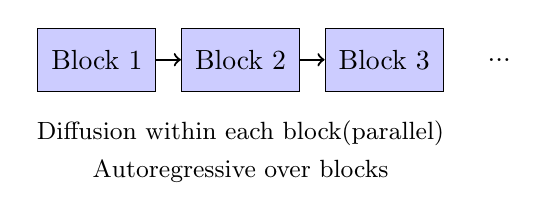
\begin{tikzpicture}[scale=0.73]
                        \node[
                            draw,
                            fill=blue!20,
                            minimum width=1.5cm,
                            minimum height=0.8cm
                        ] (b1) at (0,0) {Block 1};
                        \node[
                            draw,
                            fill=blue!20,
                            minimum width=1.5cm,
                            minimum height=0.8cm
                        ] (b2) at (2.5,0) {Block 2};
                        \node[
                            draw,
                            fill=blue!20,
                            minimum width=1.5cm,
                            minimum height=0.8cm
                        ] (b3) at (5,0) {Block 3};
                        \node (dots) at (7,0) {...};
        
                        \draw[->, thick] (b1) -- (b2) node[midway, above] {};
                        \draw[->, thick] (b2) -- (b3) node[midway, above] {};
        
                        \node[below=0.25cm of b2, align=center]
                            {\small Diffusion within each block(parallel)};
                        \node[below=0.75cm of b2, align=center]
                            {\small Autoregressive over blocks};
                    \end{tikzpicture}
                \end{center}
            \end{column}
            \begin{column}{0.4\textwidth}
                \textbf{Parameterization:} Trade-off through block size $L'$: 
                \begin{itemize}
                    \item $L' = 1$ → Pure AR
                    \item $L' = L$ → Pure Diffusion %L is inpurt size%
                \end{itemize}
            \end{column}
        \end{columns}
        \vspace{0.4cm}
        \textbf{Technical Contribution:}
        \begin{itemize}
            \item Optimized training and sampling algorithms
            \item Introduced clipped noise schedules for reduced gradient variance during training
            \item SoTA PPL among diffusion models + Variable length generation capabilities
        \end{itemize}
    \end{frame}

    
    \section{Our Results}

    \subsection{Reproduction}

    % ---------------- Reproduction Tables ----------------
    
    \begin{frame}{AR vs BD3LM with L'=1}
    
    % ---------- ROW 1 ----------
    \begin{minipage}{\textwidth}
        \begin{minipage}{0.45\textwidth}
            \centering
            \begin{table}
                \small
                \centering
                Test Perplexities for single token generation
                
                \vspace{0.2cm}
                \ra{1.2} 
                \setlength{\tabcolsep}{0.2pt}
                
                \begin{tabular}{lc}
                    \toprule
                      & PPL ($\downarrow$) \\
                    \midrule
                    $\textbf{Autoregressive}$ & \textbf{1893}\\
                    \midrule
                    $\text{\textbf{BD3LM} L'=1}$ & 2231\\
                    \midrule
                    $\text{\textbf{BD3LM} L'=1 + Tuned Schedule}$ & 2220\\
                    \bottomrule
                \end{tabular}
            \end{table}
        \end{minipage}
        \hfill
        \begin{minipage}{0.47\textwidth}
            \centering
            \includegraphics[width=\linewidth]{fig1.png}
            
            \small AR
        \end{minipage}
    \end{minipage}
    
    \vspace{0.5cm}
    
    % ---------- ROW 2 ----------
    \begin{minipage}{\textwidth}
        \centering
        \begin{minipage}{0.47\textwidth}
            \centering
            \includegraphics[width=\linewidth]{fig2.png}
            
            \small BD3LM
        \end{minipage}
        \hfill
        \begin{minipage}{0.47\textwidth}
            \centering
            \includegraphics[width=\linewidth]{fig3.png}
            
            \small BD3LM + Tuned Schedule
        \end{minipage}
    \end{minipage}
    
    \end{frame}
    
    
    \begin{frame}{The Effect of Clipped Noise Schedules}
        \begin{table}
            \centering
            \small
            \setlength{\tabcolsep}{6pt}
            \renewcommand{\arraystretch}{1.1}

            \begin{tabular}{l l c c}
                \toprule
                L' & Clipping & PPL & Var.\ NELBO \\
                \midrule
                \multirow{2}{*}{128} & U [0, 0.5] & 1000 & 1000 \\
                                     & U [0, 1]   & 1000 & 1000 \\
                \midrule
                \multirow{2}{*}{16}  & U [0.3, 0.8] & 1000 & 1000 \\
                                     & U [0, 1]     & 1000 & 1000 \\
                \midrule
                \multirow{2}{*}{4}   & U [0.5, 1] & 1226.46 & 44.41 \\
                                     & U [0, 1]   & 1225.99 & 44.41 \\
                \bottomrule
            \end{tabular}
        \end{table}
    \end{frame}
    
    \begin{frame}{Table 3}
        \centering
        \Large Table 3 Results
    \end{frame}
    
    \begin{frame}{Table 4}
        \centering
        \Large Table 4 Results
    \end{frame}
    
    \begin{frame}{Table 5}
        \centering
        \Large Table 5 Results
    \end{frame}
    
    \begin{frame}{Table 6}
        \centering
        \Large Table 6 Results
    \end{frame}
    
    \begin{frame}{Table 7}
        \centering
        \Large Table 7 Results
    \end{frame}
    
    \begin{frame}{Table 8}
        \centering
        \Large Table 8 Results
    \end{frame}


    \subsection{Extensions}

    % ---------------- New Extension Slides ----------------

    \begin{frame}{Exploring New Schedules}
        \begin{itemize}
            \item Motivation for designing alternative noise schedules
            \item Trade-off between stability and generation quality
            \item Impact on gradient variance
            \item Compatibility with block diffusion framework
        \end{itemize}
    \end{frame}
    
    \begin{frame}{New Schedules' Results}
        \begin{itemize}
            \item Comparison with cosine and clipped schedules
            \item Effects on perplexity
            \item Training stability observations
            \item Sampling behavior differences
        \end{itemize}
    \end{frame}
    

    \begin{frame}{Reweighted Losses for Improved Diffusion Objective}
        \begin{figure}
            \centering
            \includegraphics[width=\linewidth]{reweighting.png}
        \end{figure}
    \end{frame}

    \begin{frame}{Reweighted Losses for Masked Diffusion}
        \begin{itemize}
            \item Initial Reweighted NELBO:
            $$\cL^{\tilde{w}}(\bx) = -\int_0^1  \textcolor{red}{\tilde{w}(\textcolor{black}{t})}\frac{\alpha_t'}{1 - \alpha_t}\E_{q(\bz_t|\bx)}\left[\delta_{\bz_t, m}\cdot \bx^\top \log \mu_\theta(\bz_t)\right] \diff t$$
            \item Reparameterization trick: $\lambda(t) = \log \frac{\alpha_t}{1 - \alpha_t}$:
            $$\cL^{\hat{w}}(\bx) = -\int_0^1  \textcolor{blue}{\hat{w}(\textcolor{black}{\lambda(t)})}\frac{\alpha_t'}{1 - \alpha_t}\E_{q(\bz_t|\bx)}\left[\delta_{\bz_t, m}\cdot \bx^\top \log \mu_\theta(\bz_t)\right] \diff t$$
        \end{itemize}
        \begin{table}[t] 
            \centering
            % \caption{Weighting functions investigated for masked diffusion models. All functions, excluding the simple weighting, were migrated from continuous diffusion weightings by matching $\hat{w}(\lambda)$. Note that only the sigmoid, flow matching (FM), and simple weightings satisfy the necessary monotonicity requirement when paired with the cosine schedule $\alpha_t = 1 - \cos(\frac{\pi}{2}(1 - t))$.}
           % \vskip 0.1in
            \footnotesize
            \begin{tabular}{lcccc}
                \toprule
                Name  & $\lambda(t)$ & $\hat{w}(\lambda)$ & $\tilde{w}(t)$  \\
                \midrule
                EDM & \multirow{5}{*}{$\log \frac{\alpha_t}{1 - \alpha_t}$} &  $p_{\mathcal{N}(2.4, 2.4^2)}(\lambda)\frac{e^{-\lambda} + 0.5^2}{0.5^2}$ & $w(\lambda(t))$ \\ [4pt]
                IDDPM  &  & $\mathrm{sech}(\frac{\lambda}{2})$ & $2\sqrt{\alpha_t(1 - \alpha_t)}$ \\ [4pt]
                Sigmoid &  &  $\mathrm{sigmoid}(-\lambda + k)$ & $\frac{1-\alpha_t}{1 - (1 - e^{-k})\alpha_t}$ \\ [4pt]
                FM &  &  $e^{-\frac{\lambda}{2}}$ & $\sqrt{\frac{1 - \alpha_t}{\alpha_t}}$  \\ [4pt]
                Simple &  &  - & $-\frac{1 - \alpha_t}{\alpha_t'}$  \\
                \bottomrule
            \end{tabular}
        \end{table}
    \end{frame}

    \begin{frame}{Reweighted Losses Results}
    \begin{table}
        \small
        \centering
        Extended Table 3: Test Perplexities
        
        \vspace{0.2cm}
        \ra{1.2} 
        \setlength{\tabcolsep}{2pt}
        
        \begin{tabular}{lcccccc}
            \toprule
              & PPL ($\downarrow$) \\
            \midrule
            \multicolumn{2}{l}{\textbf{Autoregressive}} \\
            $\text{Transformer}$ & 1221\\
            \midrule
            \multicolumn{2}{l}{\textbf{Diffusion}} \\
            SEDD & 1403\\
            MDLM & 1370\\
            \midrule
            % UPDATED LINE BELOW
            \textbf{Block diffusion} & \textbf{Base} & \textbf{IDDPM} & \textbf{EDM} & \makecell{\textbf{Sigmoid} \\ \textbf{(k = 0)}} & \textbf{FM} & \textbf{Simple}\\
            BD3-LMs         $L'=16$  & 1345 & 252 & 49.88 & 36.06 & 76213 & 53070\\ 
            \hspace{4.1em} $L'=8$    & 1210 & 249 & 49.14 & 35.79 & 109169 & 36010741760\\
            \hspace{4.1em} $L'=4$    & 1176 & 246 & 49.01 & \textbf{35.08} & 67332 & 2396260\\
            \bottomrule
        \end{tabular}
    \end{table}
\end{frame}
    
    \section{Conclusion \& Future Work}
    
    
    
    \section{Team Organization}
    
    
    
    \section{Retrospection}

    
    
\end{document}